\documentclass[11pt]{article}
\usepackage[utf8]{inputenc}
\usepackage[T1]{fontenc}
\usepackage{mathptmx}
\usepackage[margin=1in]{geometry}
\usepackage{amsmath}
\usepackage{graphicx}
\usepackage{booktabs}
\usepackage{tabularx}
\usepackage{array}
\usepackage{multirow}
\usepackage[table]{xcolor}
\usepackage[font=small,labelfont=bf]{caption}
\usepackage{float}
\usepackage{parskip}
\usepackage{listings}
\usepackage[colorlinks=true,urlcolor=blue!60!black,linkcolor=black,citecolor=black]{hyperref}

\setlength{\parskip}{4pt}
\setlength{\textfloatsep}{10pt plus 2pt minus 2pt}\setlength{\floatsep}{8pt plus 2pt minus 2pt}\renewcommand{\topfraction}{0.9}\renewcommand{\textfraction}{0.1}\renewcommand{\floatpagefraction}{0.8}
\renewcommand{\arraystretch}{1.12}
\newcommand{\src}[1]{{\footnotesize\textit{Source:} #1}}

\lstset{basicstyle=\ttfamily\scriptsize, breaklines=true, columns=fullflexible, keepspaces=true,
  numbers=left, numberstyle=\tiny\color{gray}, numbersep=5pt, frame=single, rulecolor=\color{gray!40},
  commentstyle=\color{gray!70!black}, showstringspaces=false, upquote=true,
  literate={á}{{\'a}}1 {é}{{\'e}}1 {í}{{\'i}}1 {ó}{{\'o}}1 {ú}{{\'u}}1 {Á}{{\'A}}1 {ñ}{{\~n}}1}

\begin{document}

\begin{center}
{\LARGE\bfseries Forecasting Euro Area HICP Inflation for October 2026}\\[8pt]
{\large Álvaro Cavero Miguel}\\[3pt]
Econ 460: Economic Forecasting, University of Wisconsin--Madison \quad·\quad November 3, 2026
\end{center}

\begin{abstract}
\noindent I forecast euro area HICP annual inflation for October 2026, which Eurostat will publish on November 18, 2026. Instead of modelling the annual rate directly, I model the monthly change in the price index with monthly dummies and an autoregression, and rebuild the annual rate from the forecast index. The model is chosen by a rule set in advance: among 30 candidates, I discard those whose residuals fail the Box-Pierce test and pick the lowest BIC. The rule selects an AR(13) with fixed seasonal dummies. In a recursive out-of-sample exercise since 2015 it has the lowest root mean squared prediction error at every horizon against an AR and an ARMA for the annual rate and the random walk, although the gains at one month are small. Alternative specifications give October forecasts between 4.01\% and 4.15\%. My forecast is 4.1\%, with a 50\% interval of 3.9\% to 4.3\% and a 90\% interval of 3.5\% to 4.7\%.
\end{abstract}

%=====================================================================
\section{Introduction}

The euro area inflation rate is the variable that the European Central Bank (ECB) targets, with a goal of 2\% over the medium term. After two years close to that goal, inflation rose during 2026, from 1.7\% in January to 3.8\% in September, mostly because of higher energy prices. In September energy prices were 18.9\% higher than a year earlier, while services inflation was 3.2\% (Eurostat, 2026a). This makes the next few months hard to predict.

The target of this paper is the \emph{final} October 2026 figure, which Eurostat releases on its website on Wednesday, November 18, 2026. A flash estimate comes out earlier, on November 4. This report is written before both releases, with data up to September 2026, so the forecast is one month ahead ($h=1$).

The annual inflation rate is approximately the sum of the last twelve monthly price changes, and for October 2026 eleven of those twelve months are already known. So I forecast only the missing month, the change in prices from September to October, and rebuild the annual rate from the price index. Section~\ref{sec:data} describes the data. Section~\ref{sec:model} presents the model and the rule I use to choose it. Section~\ref{sec:est} reports the estimates and the residual checks, and Section~\ref{sec:oos} evaluates the rule out of sample. Section~\ref{sec:fc} gives the forecast and the intervals, Section~\ref{sec:others} compares them with other forecasts, and Section~\ref{sec:concl} discusses limitations.

%=====================================================================
\section{The data}
\label{sec:data}

\subsection{The variable}

The HICP is a price index for a fixed basket of goods and services bought by households in the euro area, with base year 2025 = 100. Eurostat publishes it every month. I use the dataset \texttt{prc\_hicp\_minr} (all items, euro area with changing composition), downloaded with the R package \texttt{eurostat}. I take two series: the official annual rate of change and the index itself. The changing composition series is the headline figure; it includes each country from the month it joined the euro, so Bulgaria is included from January 2026. Since 2026 Eurostat also compiles the HICP with a new classification of products (ECOICOP version 2) and has recalculated the whole history on that basis.

The annual inflation rate in month $t$ is
\begin{equation}
\pi_t = 100\left(\frac{P_t}{P_{t-12}}-1\right),
\label{eq:yoy}
\end{equation}
where $P_t$ is the price index. Figure~\ref{fig:series} plots it from January 1997 to September 2026 (357 observations). The sample mean is 2.07\%. Inflation stayed close to 2\% until 2008, was negative in 2009 and around 2015, and reached a peak of 10.6\% in October 2022 during the energy crisis. It fell back to about 2\% in 2024-25 and has been rising again in 2026.

\begin{figure}[htbp]
\centering
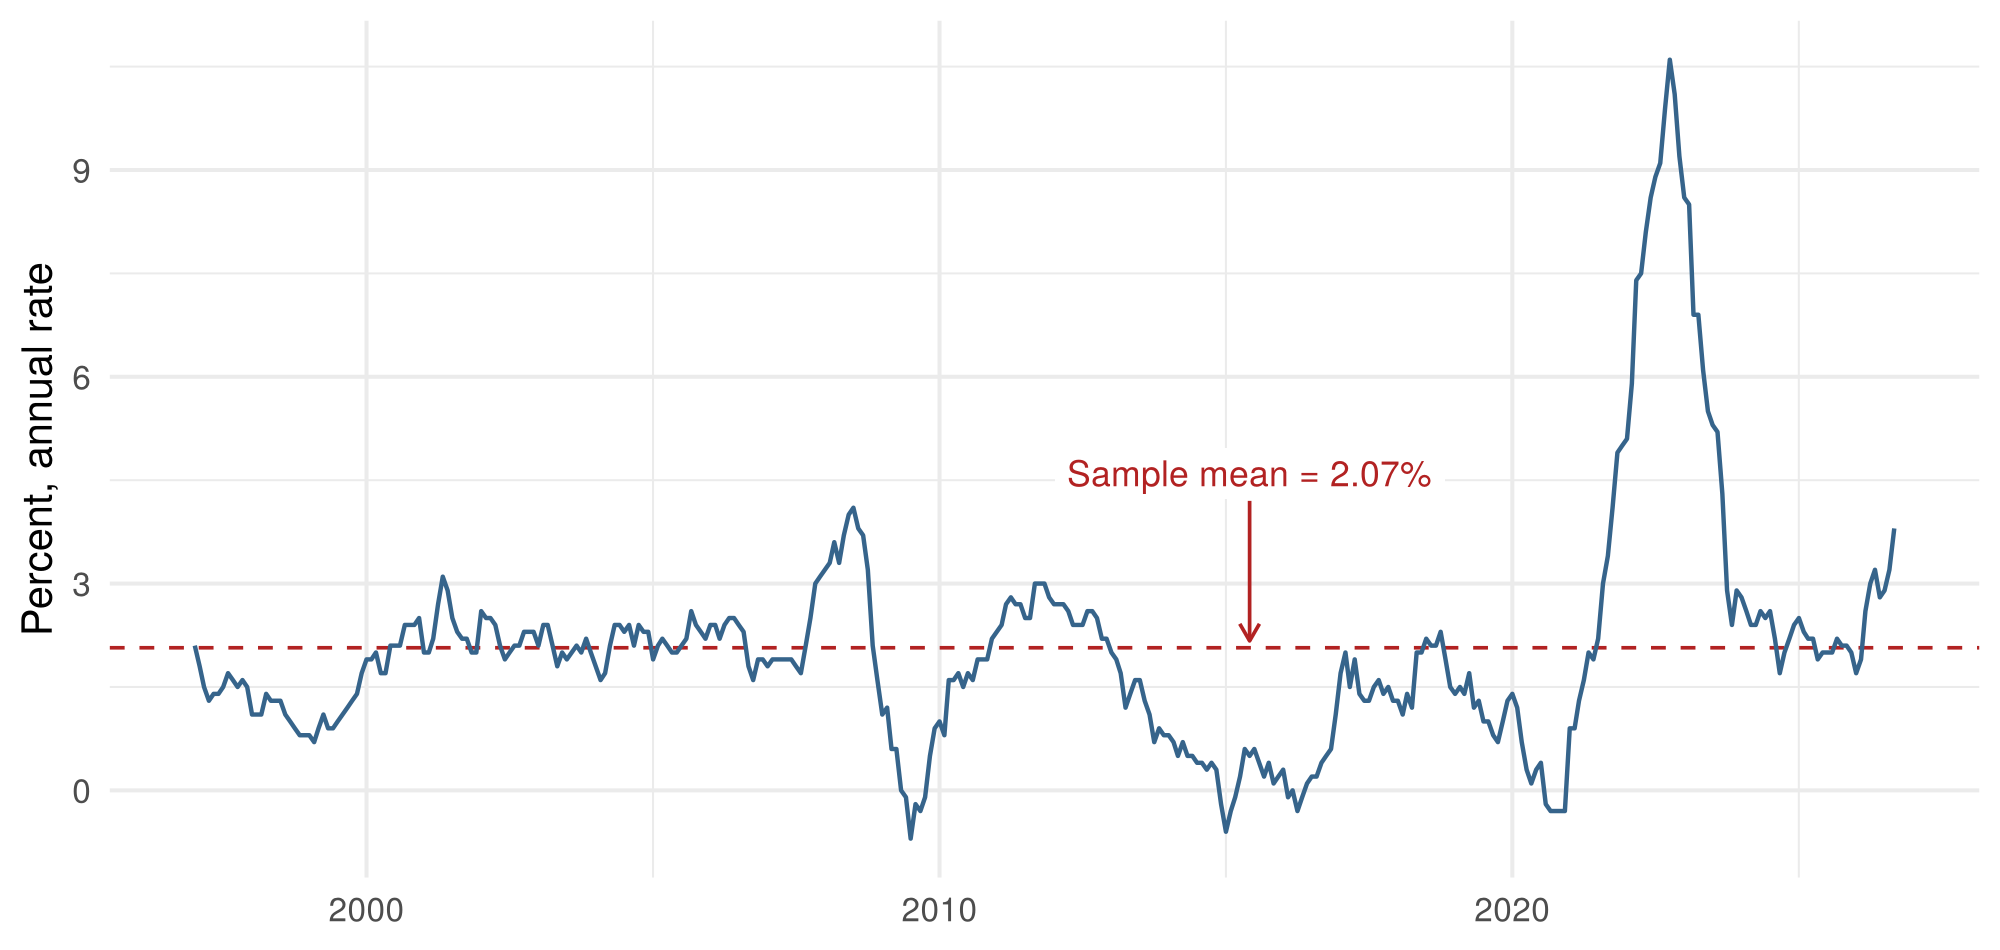
\includegraphics[width=0.85\textwidth]{fig/fig_series.png}
\caption{Euro area HICP inflation, annual rate (\%), January 1997 to September 2026. The dashed line is the sample mean, 2.07\%.}
\label{fig:series}
\end{figure}
\vspace{-6pt}
\src{Eurostat, \href{https://ec.europa.eu/eurostat/databrowser/view/prc_hicp_minr/default/table}{\texttt{prc\_hicp\_minr}}, retrieved with the R package \texttt{eurostat}; figure by the author.}

\subsection{Annual rate and monthly changes}

Define the monthly change in prices, in percent, as the log difference of the index:
\begin{equation}
m_t = 100\,(\ln P_t - \ln P_{t-1}).
\label{eq:mm}
\end{equation}
Because log changes add up, $\ln(P_t/P_{t-12})$ is the sum of the last twelve monthly log changes, so
\begin{equation}
\pi_t \approx m_t + m_{t-1} + \dots + m_{t-11}
\qquad\text{and}\qquad
\pi_t - \pi_{t-1} \approx m_t - m_{t-12}.
\label{eq:sum}
\end{equation}
The second expression is the \emph{base effect}: the annual rate goes up when this month's price change is larger than the change in the same month one year earlier. For my target this means that October 2026 inflation will be above September's 3.8\% if prices rise more from September to October 2026 than they did from September to October 2025, when they rose by 0.22\%. With the index I can check that the official rate and the rate computed with \eqref{eq:yoy} differ by at most 0.05 points, which is the rounding to one decimal. The monthly series starts in February 1997 (356 observations).

\subsection{What the data show}

Figure~\ref{fig:acf} shows the autocorrelation (ACF) and partial autocorrelation (PACF) functions of both series. The annual rate is very persistent. Its first autocorrelation is 0.98 and the ACF dies out very slowly, which is what \eqref{eq:sum} predicts, since two consecutive annual rates share eleven of their twelve monthly terms. Its PACF has a large spike at lag 13 (0.31). This is the base effect again, a result of how the annual rate is built.

The monthly change looks very different. Its first autocorrelation is only 0.15, but there are large spikes at lags 12, 24 and 36 (0.73 at lag 12) and smaller ones at lags 6, 18 and 30. This is strong seasonality. Prices fall in January and July because of the winter and summer sales and rise in March, when new collections arrive. Months that are six months apart, like the two sales months, also look alike.

\begin{figure}[htbp]
\centering
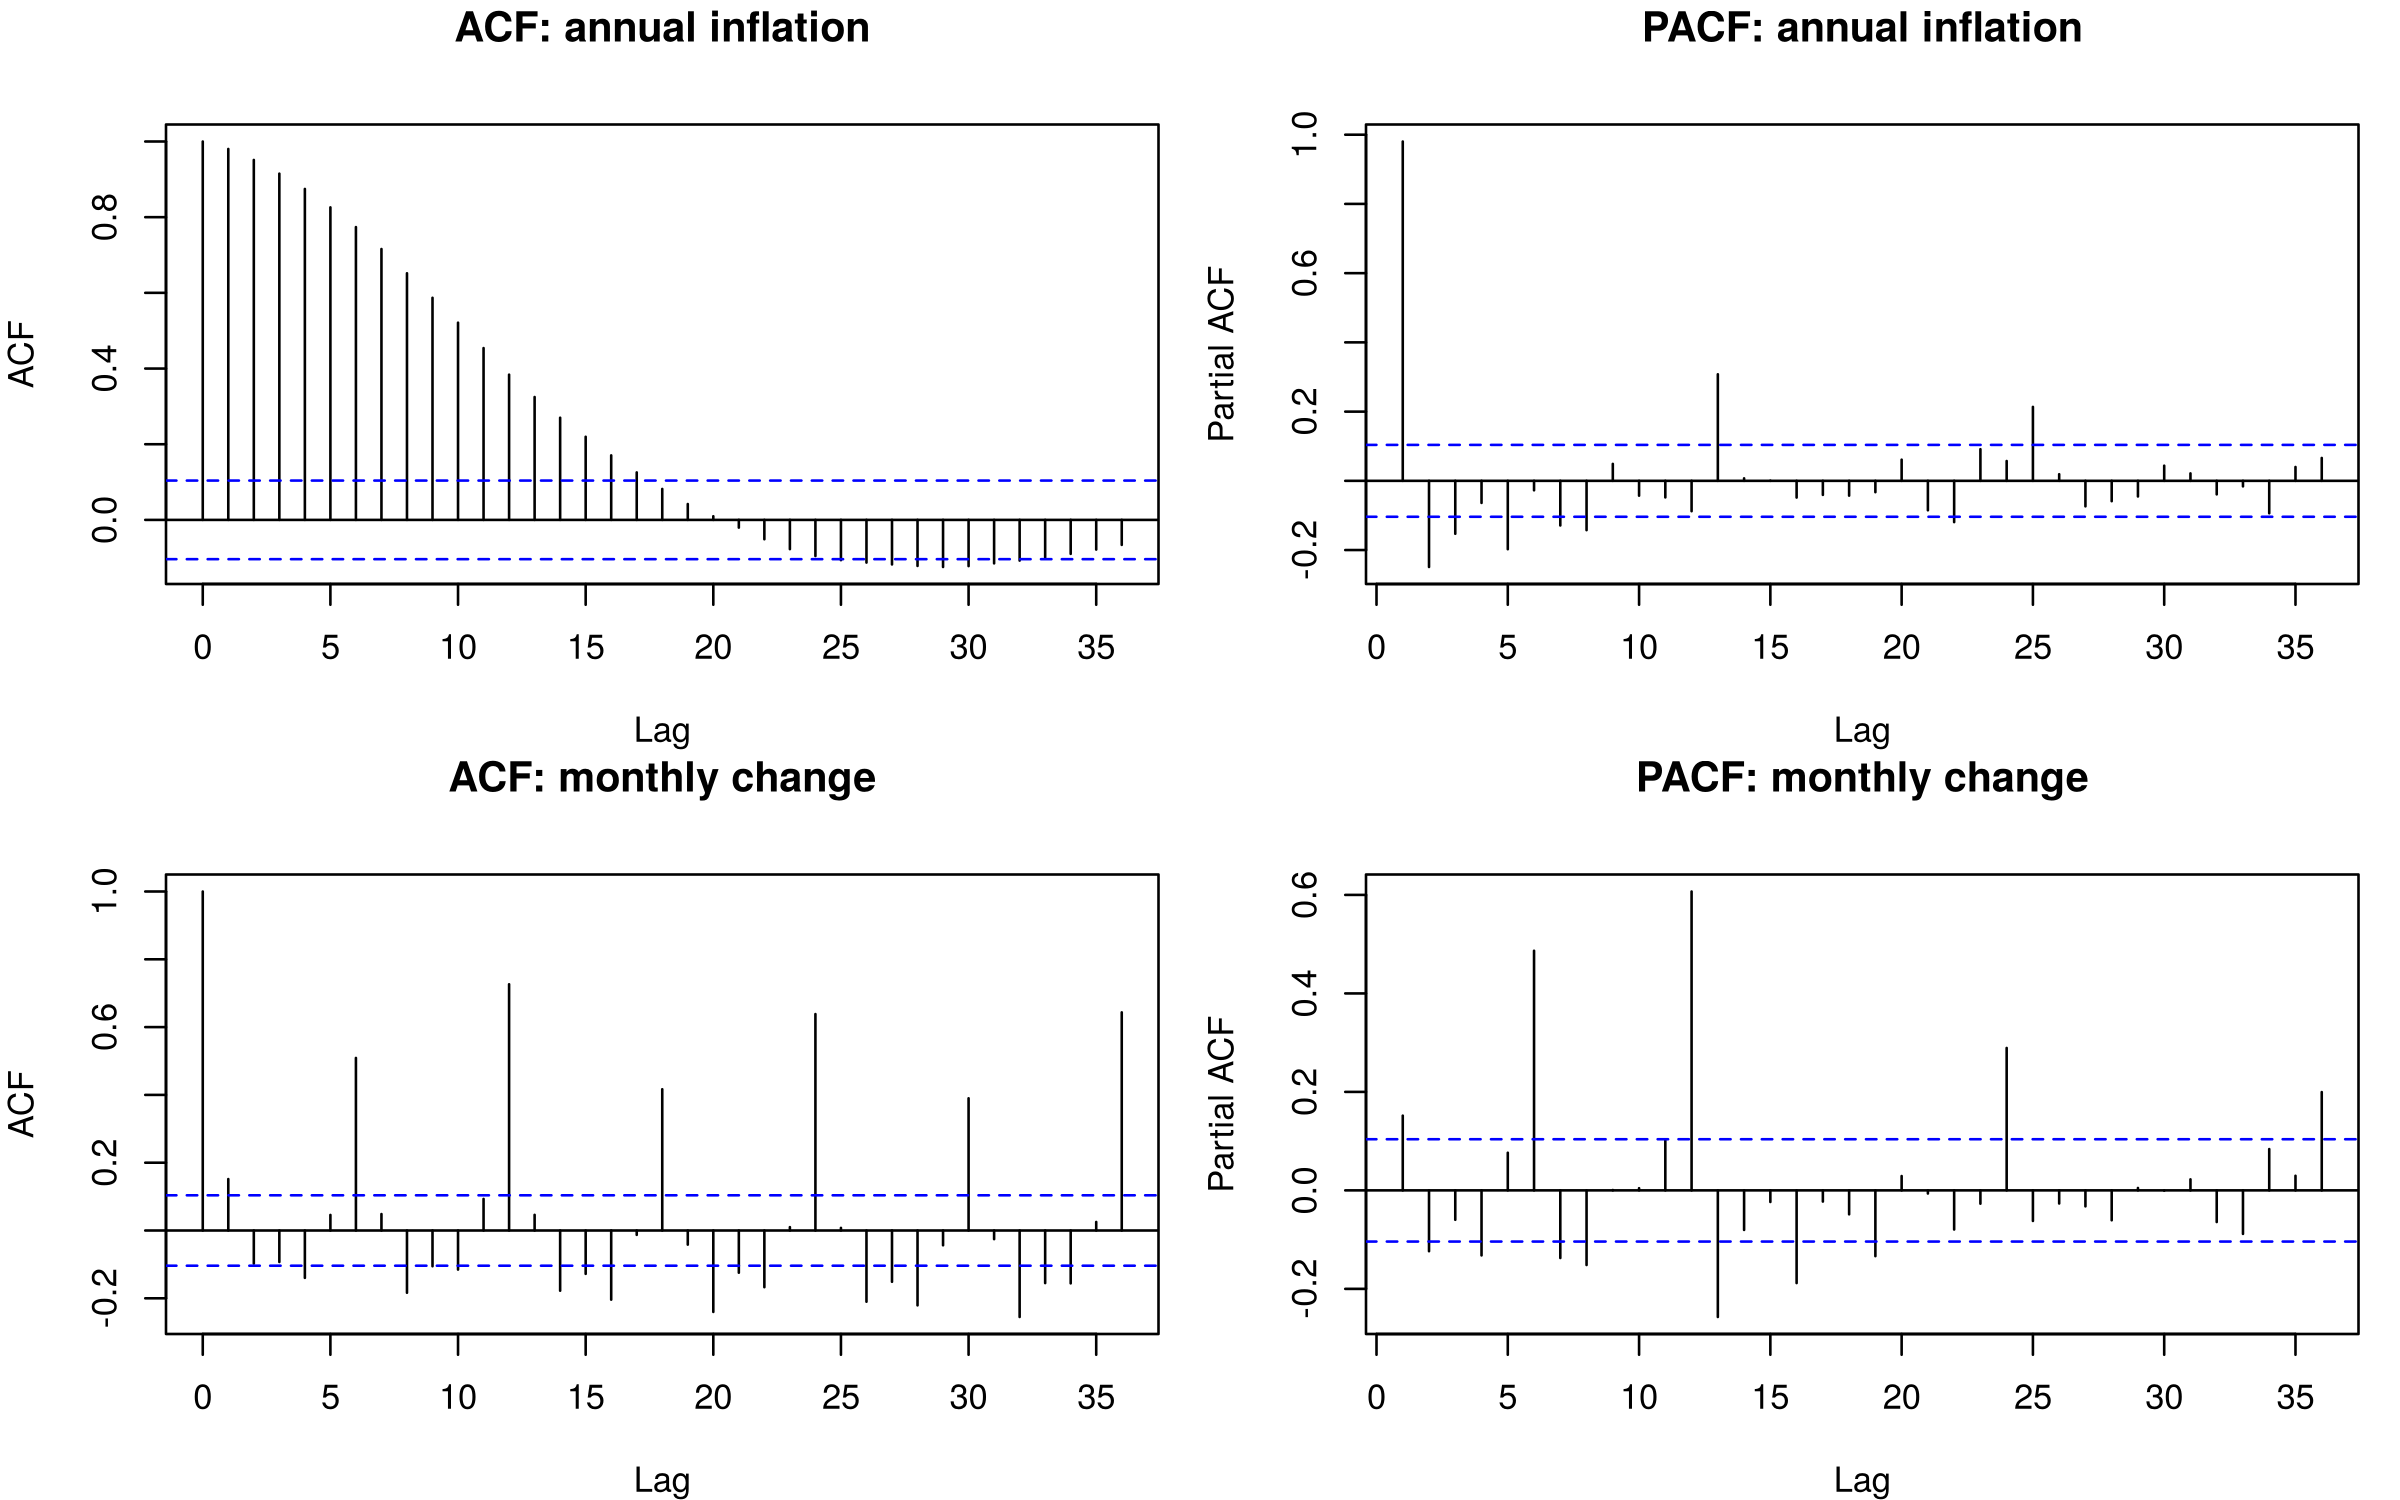
\includegraphics[width=0.8\textwidth]{fig/acf_pacf.png}
\caption{ACF and PACF of the annual inflation rate (top) and of the monthly change (bottom). The dashed bands are $\pm1.96/\sqrt{T}$.}
\label{fig:acf}
\end{figure}

The seasonal pattern has also changed over time. Figure~\ref{fig:season} compares the average monthly change of each calendar month before and after 2011. Since 2011 January prices fall more ($-0.72\%$ on average against $-0.34\%$ before) and March prices rise more (1.09\% against 0.53\%). A likely reason is Commission Regulation (EC) No 330/2009, which set common rules for recording the prices of seasonal products such as clothing and footwear in the HICP and was applied from 2011. Following the advice of the course not to mix different regimes in one sample, the model has to allow for this change in some way. Section~\ref{sec:model} explains how.

\begin{figure}[htbp]
\centering
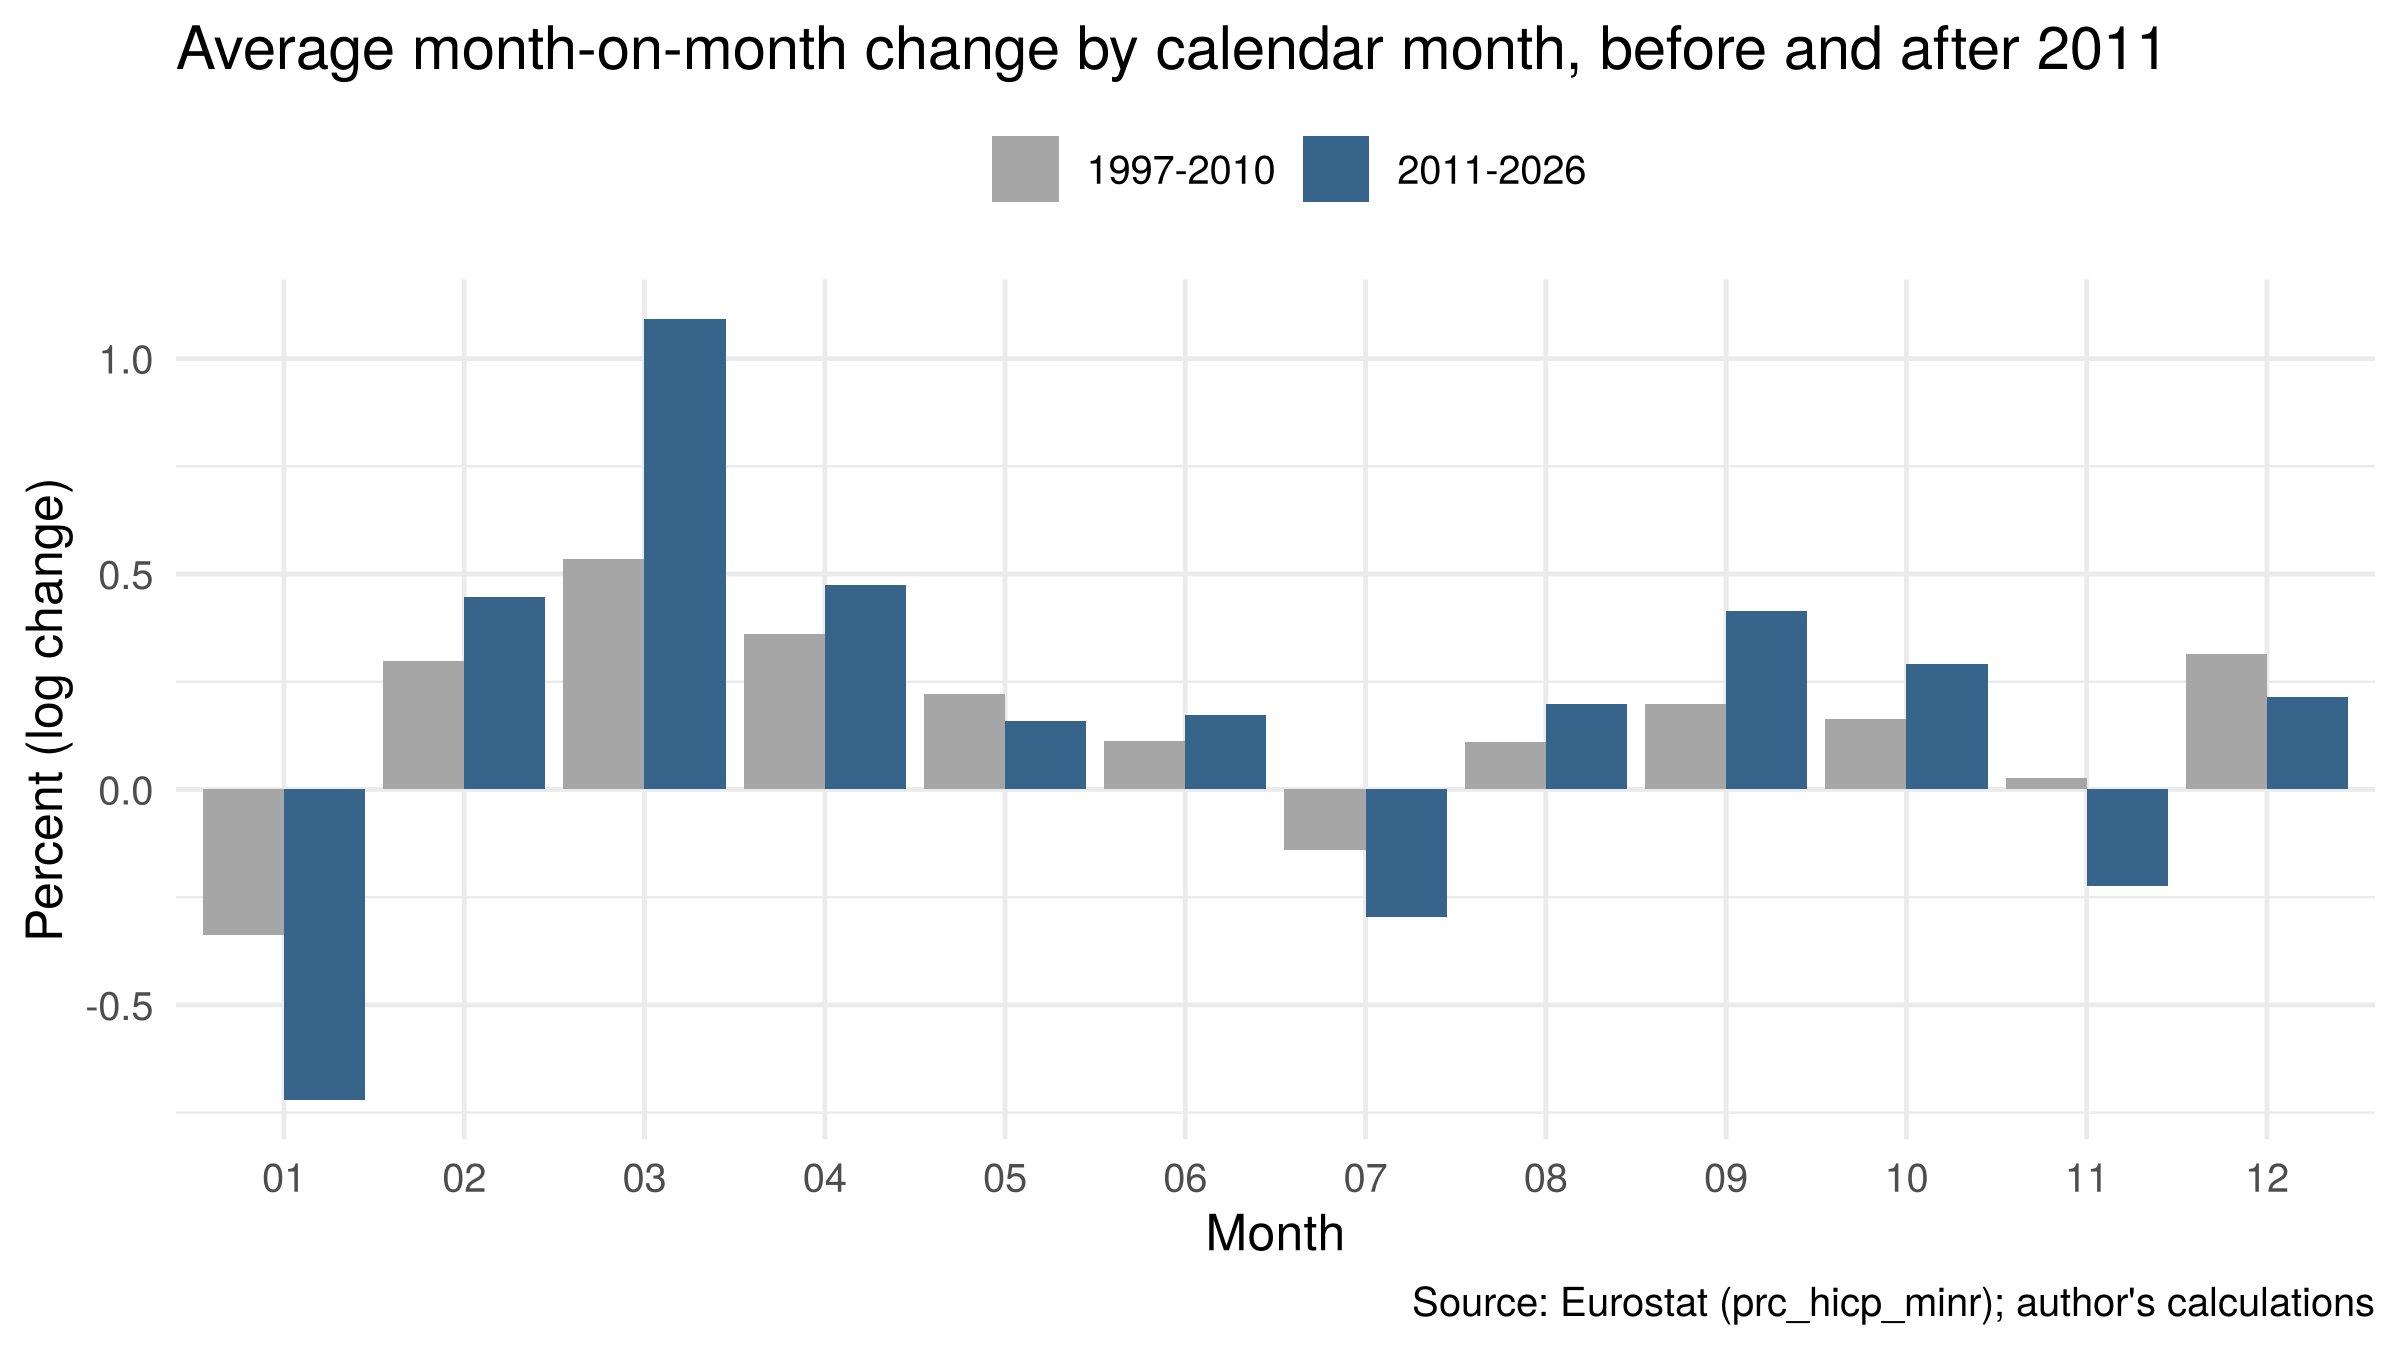
\includegraphics[width=0.72\textwidth]{fig/seasonality_by_period.png}
\caption{Average monthly change in the HICP by calendar month, 1997-2010 and 2011-2026.}
\label{fig:season}
\end{figure}

%=====================================================================
\section{The model and how I chose it}
\label{sec:model}

\subsection{A seasonal autoregression for the monthly change}

Based on Section~\ref{sec:data}, I model the monthly change with monthly dummies and $p$ of its own lags:
\begin{equation}
m_t = \beta_0 + \sum_{j=\text{Feb}}^{\text{Dec}} \delta_j D_{jt} + \phi_1 m_{t-1} + \dots + \phi_p m_{t-p} + \varepsilon_t ,
\label{eq:model}
\end{equation}
where $D_{jt}=1$ if month $t$ is calendar month $j$. January is the base month, so there are 11 dummies and $\delta_j$ measures how much more prices change in month $j$ than in January. The model is estimated by OLS. As shown in lecture 12, estimating the seasonal dummies and the AR terms in one regression gives the same result as first removing the seasonal means and then fitting an AR to what is left.

The forecast of $m$ comes from the chain rule of forecasting: for $h=1$ all terms on the right of \eqref{eq:model} are known, and for $h>1$ the forecasts of earlier months replace the unknown values. The forecast index is $\ln\hat P_{T+h} = \ln P_T + \frac{1}{100}\sum_{j=1}^{h}\hat m_{T+j}$, and the forecast of the annual rate is
\begin{equation}
\hat\pi_{T+h} = 100\left(\frac{\hat P_{T+h}}{P_{T+h-12}}-1\right).
\label{eq:rebuild}
\end{equation}
For $h\le12$ the denominator is already observed, so the base effect enters the forecast automatically. For October 2026 it is the index of October 2025.

There are two ways to let the seasonal pattern change, and I treat both as candidates.
\begin{enumerate}
\item \emph{A break in 2011.} Add a dummy $\text{Post}_t$ equal to 1 from January 2011 and its interactions with the 11 monthly dummies. Each month then has one seasonal effect before 2011 and another one after, while the AR coefficients are estimated with the full sample. This costs 12 extra parameters, and the break date is chosen by me.
\item \emph{Seasonal lags.} Allow $p$ to be 12 or more. The lag $m_{t-12}$ is the change in the same month of the previous year. If the pattern of a month drifts over time, last year's value of that month is more informative than its 30-year average, and the coefficient on $m_{t-12}$ picks this up without fixing any date. In the data, after removing each month's average, the monthly change is correlated with its value 12 months earlier (correlation 0.39), so this information exists.
\end{enumerate}
To make the second option possible, the maximum lag length must be at least a year. I use $p_{\max}=14$. A first version of the model used $p_{\max}=6$, the default suggested in lecture 10, but the BIC then chose $p=6$, the upper limit, which is a sign that the limit was too low.

\subsection{The selection rule}

I want the data to decide between these options, so I fixed a rule before looking at which model wins. It follows the Box-Jenkins steps of lecture 9 and the information criteria of lecture 10, and it is the same logic as the course example on U.S.\ inflation, where an AR(1) is rejected because its residuals fail the Box-Pierce test and an AR(2) passes and is also preferred by AIC and BIC.

\begin{enumerate}
\item \emph{Candidates.} Fixed seasonals or the 2011 break, combined with $p=0,1,\dots,14$: 30 models. All are estimated on the same sample (342 months) so that their criteria are comparable.
\item \emph{Residual check.} Keep only the models whose residuals pass the Box-Pierce test at 5\%. The statistic is
\begin{equation}
Q = T\sum_{k=1}^{R}\hat\rho_k^{\,2}\ \sim\ \chi^2(R)\ \ \text{under white noise},
\label{eq:bp}
\end{equation}
where $\hat\rho_k$ is the $k$-th autocorrelation of the residuals and $R=\lfloor\sqrt{T}\rfloor=18$. The 5\% critical value is 28.9.\footnote{I follow the course and compare $Q$ with a $\chi^2(R)$. For the residuals of an estimated AR($p$), Box and Pierce (1970) show that the degrees of freedom should be $R-p$. With $R=18$ this leaves few degrees of freedom when $p$ is close to 18. With $R-p$ degrees of freedom the rule selects the AR(14) with fixed seasonals instead of the AR(13). Its October forecast is also 4.10\% (Table~\ref{tab:robust}).} A model that fails leaves predictable information in its errors.
\item \emph{Choice.} Among the models that pass, choose the one with the lowest
\begin{equation}
\text{BIC} = \ln\hat\sigma^2 + \frac{k\ln T}{T},
\label{eq:bic}
\end{equation}
where $\hat\sigma^2$ is the residual variance and $k$ the number of parameters. I also report $\text{AIC}=\ln\hat\sigma^2+2k/T$, but I use the BIC because it penalizes extra parameters more heavily and is the criterion recommended in the course.
\end{enumerate}

I do not use F or t tests to choose variables. A joint test can be significant because of one or two variables only, and running many tests on the same data makes it likely to find something significant by chance. The models of the annual rate (an AR and an ARMA) cannot enter the BIC comparison because they explain a different variable, so I use them as benchmarks in Section~\ref{sec:oos}.

\subsection{Results of the rule}

Table~\ref{tab:select} shows the 30 candidates and Figure~\ref{fig:bic} plots the BIC and the Box-Pierce statistic.

\begin{table}[htbp]
\centering
\small
\caption{Candidate models: information criteria and Box-Pierce test (common sample, $T=342$)}
\label{tab:select}
\setlength{\tabcolsep}{5pt}
\begin{tabular}{@{}r|rrrrc|rrrrc@{}}
\toprule
 & \multicolumn{5}{c|}{Fixed seasonal dummies} & \multicolumn{5}{c}{Seasonal dummies with 2011 break}\\
$p$ & $k$ & AIC & BIC & $Q(18)$ & Pass & $k$ & AIC & BIC & $Q(18)$ & Pass\\
\midrule
0 & 12 & $-2.466$ & $-2.332$ & 183.2 & no & 24 & $-2.549$ & $-2.280$ & 194.6 & no\\
1 & 13 & $-2.544$ & $-2.398$ & 120.1 & no & 25 & $-2.638$ & $-2.358$ & 93.4 & no\\
2 & 14 & $-2.539$ & $-2.382$ & 120.7 & no & 26 & $-2.641$ & $-2.350$ & 87.1 & no\\
3 & 15 & $-2.550$ & $-2.382$ & 105.0 & no & 27 & $-2.667$ & $-2.364$ & 58.4 & no\\
4 & 16 & $-2.546$ & $-2.367$ & 109.9 & no & 28 & $-2.667$ & $-2.353$ & 63.0 & no\\
5 & 17 & $-2.558$ & $-2.367$ & 93.4 & no & 29 & $-2.669$ & $-2.344$ & 57.9 & no\\
6 & 18 & $-2.690$ & $-2.488$ & 29.8 & no & 30 & $-2.754$ & $-2.417$ & 19.1 & yes\\
7 & 19 & $-2.684$ & $-2.471$ & 29.8 & no & 31 & $-2.748$ & $-2.400$ & 19.1 & yes\\
8 & 20 & $-2.684$ & $-2.459$ & 31.0 & no & 32 & $-2.744$ & $-2.385$ & 19.3 & yes\\
9 & 21 & $-2.678$ & $-2.443$ & 30.7 & no & 33 & $-2.740$ & $-2.370$ & 18.4 & yes\\
10 & 22 & $-2.677$ & $-2.430$ & 30.5 & no & 34 & $-2.738$ & $-2.356$ & 18.6 & yes\\
11 & 23 & $-2.680$ & $-2.422$ & 28.8 & yes & 35 & $-2.735$ & $-2.343$ & 17.5 & yes\\
12 & 24 & $-2.726$ & $-2.457$ & 17.8 & yes & 36 & $-2.742$ & $-2.339$ & 14.9 & yes\\
\rowcolor{gray!30} 13 & 25 & $-2.765$ & $\mathbf{-2.484}$ & 11.7 & yes & 37 & $-2.773$ & $-2.358$ & 10.6 & yes\\
14 & 26 & $-2.769$ & $-2.478$ & 7.5 & yes & 38 & $-2.773$ & $-2.347$ & 6.4 & yes\\
\bottomrule
\end{tabular}

\vspace{3pt}
{\footnotesize $k$: number of parameters. Pass: $Q(18)$ below the 5\% critical value of 28.9. Shaded row: selected model.}
\end{table}

\begin{figure}[htbp]
\centering
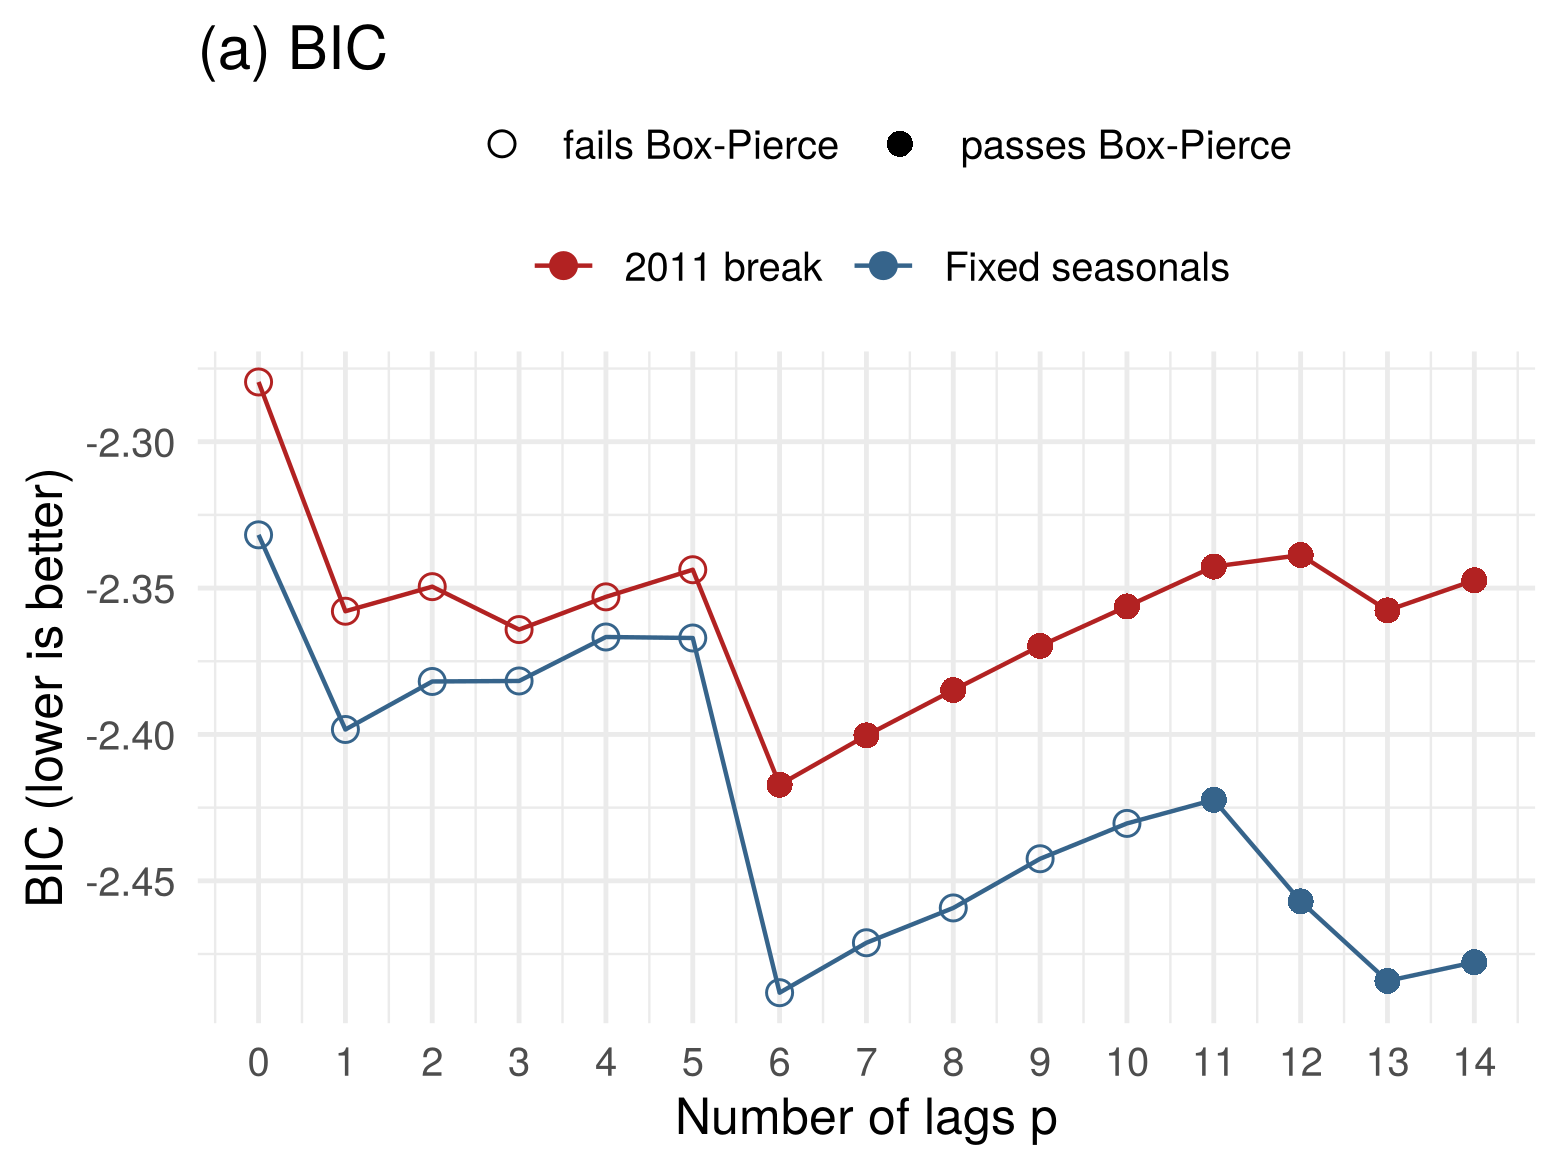
\includegraphics[width=0.49\textwidth]{fig/fig_bic.png}\hfill
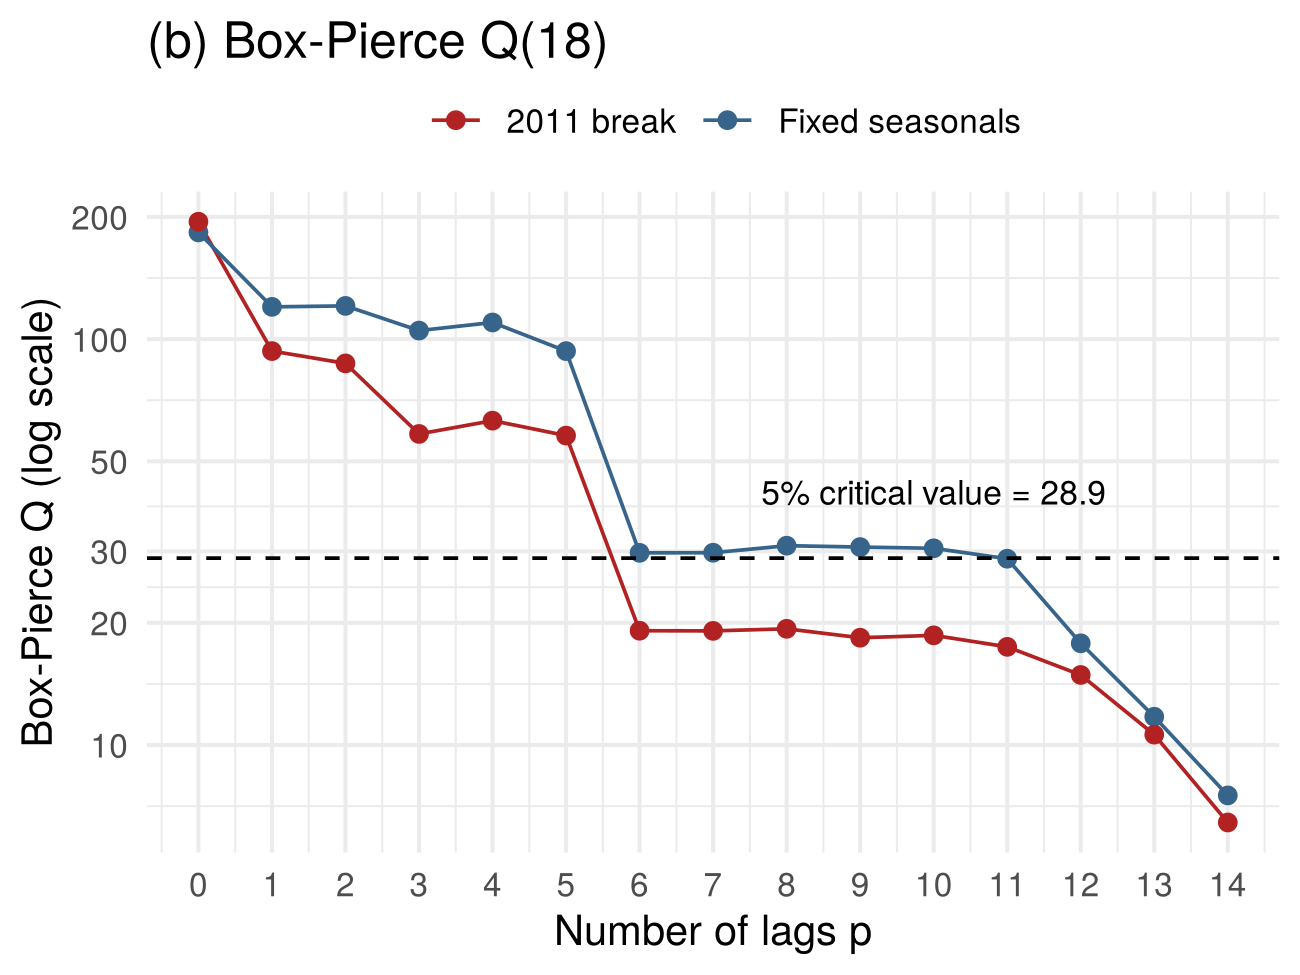
\includegraphics[width=0.49\textwidth]{fig/fig_bp.png}
\caption{BIC (a) and Box-Pierce statistic (b) of the 30 candidates. In panel (a), filled points pass the Box-Pierce test.}
\label{fig:bic}
\end{figure}

The table shows three results. First, no model with fewer than six lags passes the residual check, with or without the break. Second, the model with fixed seasonals and $p=6$ has the lowest BIC of the whole table ($-2.488$), but it fails the test ($Q=29.8>28.9$): its residuals are still correlated with the residuals of the same month one year earlier, so the rule rejects it. Third, with fixed seasonals the BIC gets worse from $p=6$ to $p=11$ and then improves again at $p=12$ and $p=13$, while $Q$ falls to 11.7. The break models pass from $p=6$ on, but their 12 extra parameters give them a clearly higher BIC (at best $-2.417$).

The selected model is therefore the seasonal AR(13) with fixed seasonal dummies. Its BIC ($-2.484$) is almost the same as the best value in the table and its residuals pass the test easily. The data agree that the seasonal pattern has changed, since with fixed seasonals a model passes the test only once it includes lags of about one year ($p\ge11$), but they prefer to capture the change with seasonal lags rather than with a break on a date that I chose.

%=====================================================================
\section{Estimates and residual checks}
\label{sec:est}

Table~\ref{tab:param} reports the estimates of the selected model on the full sample.

\begin{table}[htbp]
\centering
\small
\caption{Estimated seasonal AR(13) for the monthly change in the HICP}
\label{tab:param}
\begin{tabular}{@{}lrr@{\hspace{3em}}lrr@{}}
\toprule
Parameter & Estimate & s.e. & Parameter & Estimate & s.e.\\
\midrule
Constant (January) & $-0.354$ & 0.075 & February & 0.632 & 0.110\\
$m_{t-1}$ & 0.253 & 0.055 & March & 0.840 & 0.102\\
$m_{t-2}$ & 0.014 & 0.054 & April & 0.584 & 0.108\\
$m_{t-3}$ & 0.063 & 0.054 & May & 0.464 & 0.107\\
$m_{t-4}$ & 0.058 & 0.054 & June & 0.343 & 0.106\\
$m_{t-5}$ & $-0.006$ & 0.054 & July & 0.229 & 0.093\\
$m_{t-6}$ & 0.269 & 0.054 & August & 0.411 & 0.106\\
$m_{t-7}$ & 0.071 & 0.056 & September & 0.233 & 0.109\\
$m_{t-8}$ & $-0.094$ & 0.054 & October & 0.422 & 0.109\\
$m_{t-9}$ & 0.026 & 0.054 & November & 0.189 & 0.104\\
$m_{t-10}$ & $-0.077$ & 0.054 & December & 0.547 & 0.107\\
$m_{t-11}$ & 0.058 & 0.054 & & & \\
$m_{t-12}$ & 0.273 & 0.054 & & & \\
$m_{t-13}$ & $-0.206$ & 0.055 & & & \\
\midrule
\multicolumn{6}{@{}l}{$\hat\sigma = 0.243$ \qquad $R^2 = 0.72$ \qquad $n = 343$ (March 1998 to September 2026)}\\
\bottomrule
\end{tabular}

\vspace{3pt}
{\footnotesize OLS estimates. The dependent variable is $m_t$ in percent. Monthly dummies are relative to January.}
\end{table}

Four lags are clearly different from zero. The first lag (0.253) is the usual persistence from one month to the next. Lag 6 (0.269) links months that are half a year apart, such as the two sales periods. Lag 12 (0.273) is the seasonal lag: if prices rose one point more than usual in October 2025, the model expects them to rise about 0.27 points more than usual in October 2026. Lag 13 has a negative sign ($-0.206$). Part of last year's change came from the momentum of the month before it, and this term removes that part. The other lags are small. I keep them because the rule chooses the lag length as a whole, as in the course, and not lag by lag. All monthly dummies are positive because they are measured against January, the month of the winter sales.

Lags and dummies are moderately correlated with each other. For example, the value 12 months before an October observation is also an October value, so it carries part of the October effect. The variance inflation factors are between 3 and 5, below the usual warning level of 10. This makes individual standard errors larger, but it does not bias the forecast, and the selection rule does not use standard errors.

The residuals of the final model look like white noise (Figure~\ref{fig:resid}). Their autocorrelations at lags 1, 12 and 24 are $-0.03$, $-0.04$ and $0.00$, all inside the 95\% band of $\pm0.11$, and the Box-Pierce statistic on the full sample is $Q(18)=12.0$, far below 28.9. For comparison, the residuals of the AR(6) with fixed seasonals have an autocorrelation of 0.21 at lag 12, which is the pattern that lags 12 and 13 remove.

\begin{figure}[htbp]
\centering
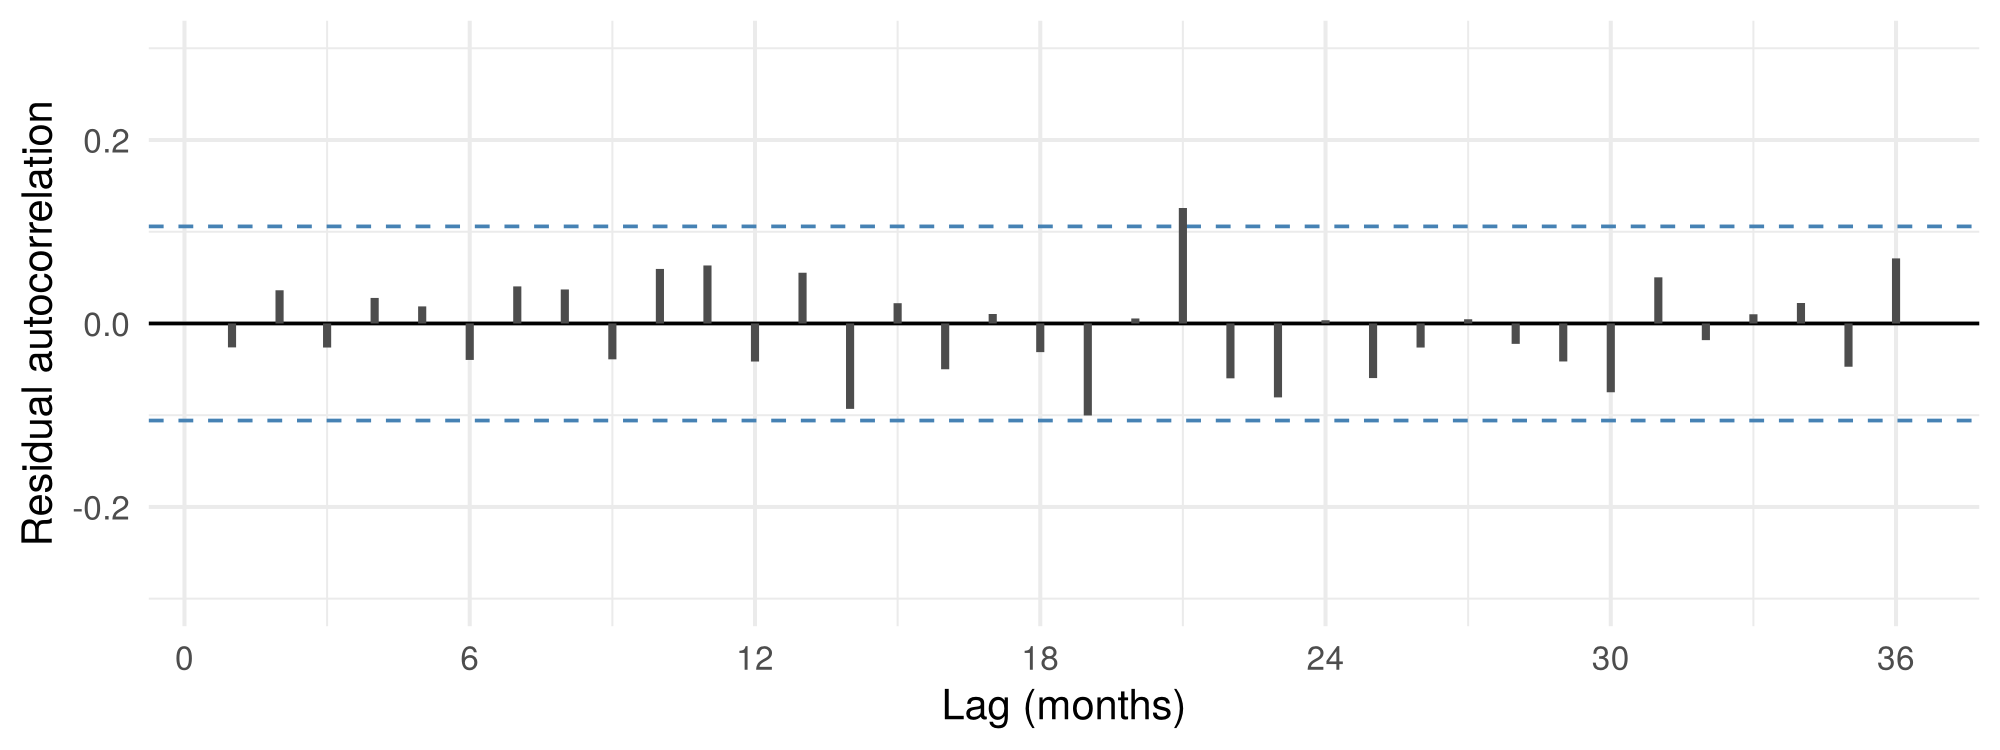
\includegraphics[width=0.8\textwidth]{fig/fig_resid.png}
\caption{Autocorrelations of the residuals of the selected model, lags 1 to 36. The dashed lines are the 95\% bands, $\pm1.96/\sqrt{343}$.}
\label{fig:resid}
\end{figure}

%=====================================================================
\section{Out-of-sample evaluation}
\label{sec:oos}

The BIC and the Box-Pierce test use the whole sample. To check how the procedure would have worked in real time, I run a recursive pseudo out-of-sample exercise, as in Handouts 2 and 4. For every month from January 2015 to August 2026 (140 forecast origins) I keep only the data up to that month, re-estimate every model and forecast the next 12 months. For the seasonal model the whole selection rule is applied again at each origin, so the choice of seasonals and lag length can change over time. I compare four models with the seasonal rule: the random walk ($\hat\pi_{T+h}=\pi_T$), the sample mean, an AR($p$) for the annual rate with $p\le13$ chosen by BIC (13 because of the PACF spike), and an ARMA(1,1) for the annual rate estimated by maximum likelihood. The forecast error is $e = \pi - \hat\pi$, and I summarise it with the root mean squared prediction error (RMSPE).

\begin{table}[htbp]
\centering
\small
\caption{Out-of-sample RMSPE of the annual inflation rate (percentage points), origins January 2015 to August 2026}
\label{tab:rmspe}
\begin{tabular}{@{}lrrrrr@{}}
\toprule
Model & $h=1$ & $h=3$ & $h=6$ & $h=12$ & $h=1$, excl.\ 2021-23\\
\midrule
Seasonal AR, selection rule & \textbf{0.354} & \textbf{0.732} & \textbf{1.246} & \textbf{2.507} & \textbf{0.259}\\
AR($p$), annual rate & 0.374 & 0.818 & 1.428 & 2.678 & 0.305\\
ARMA(1,1), annual rate & 0.407 & 0.913 & 1.578 & 2.692 & 0.291\\
Random walk & 0.421 & 0.926 & 1.589 & 2.767 & 0.296\\
Sample mean & 2.511 & 2.534 & 2.576 & 2.649 & 0.960\\
\bottomrule
\end{tabular}

\vspace{3pt}
{\footnotesize The last column drops target months from July 2021 to December 2023, the period of very high inflation.}
\end{table}

\begin{figure}[htbp]
\centering
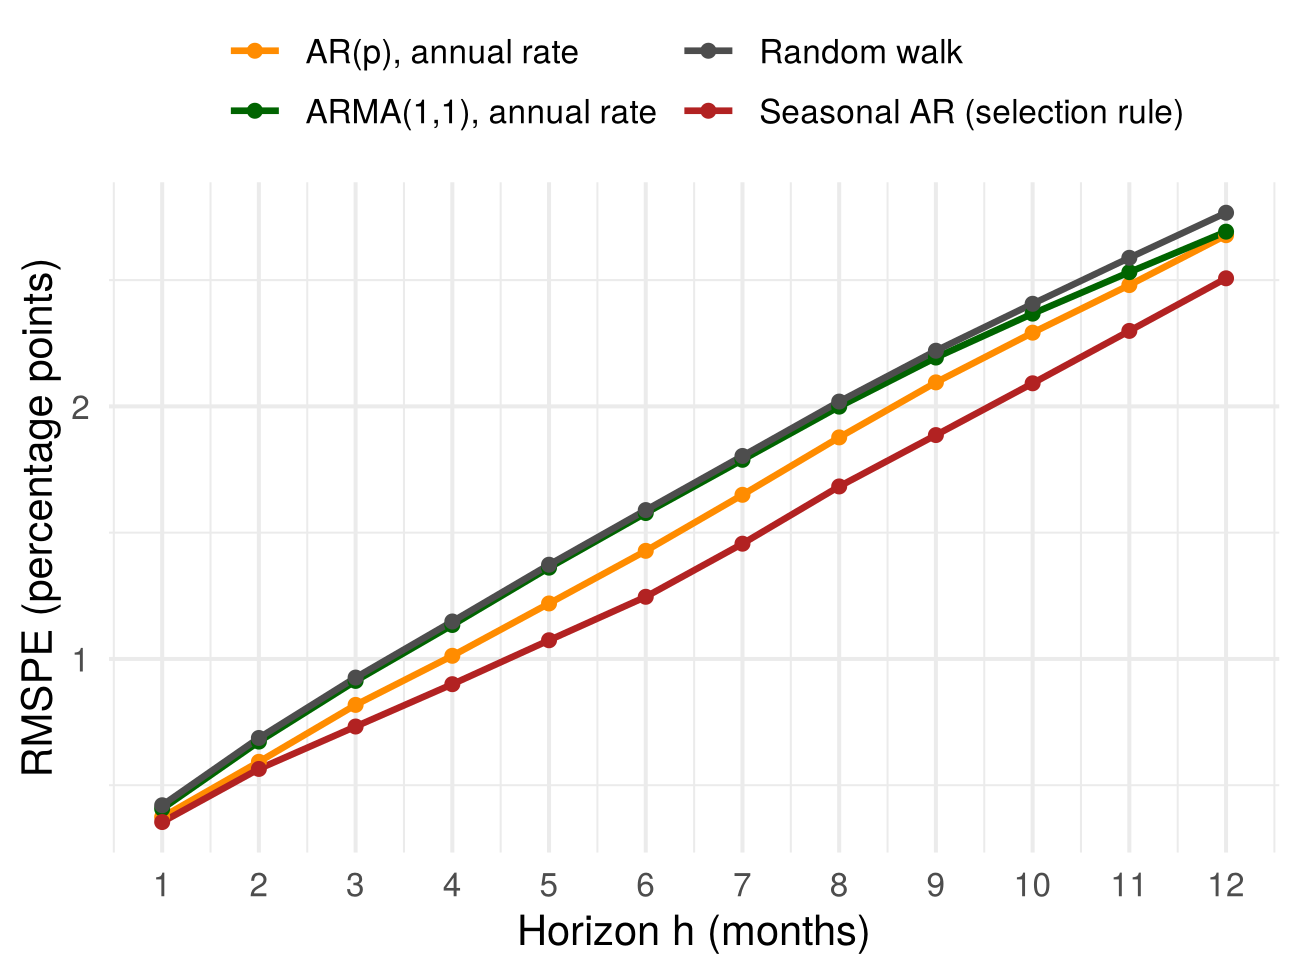
\includegraphics[width=0.49\textwidth]{fig/fig_rmspe.png}\hfill
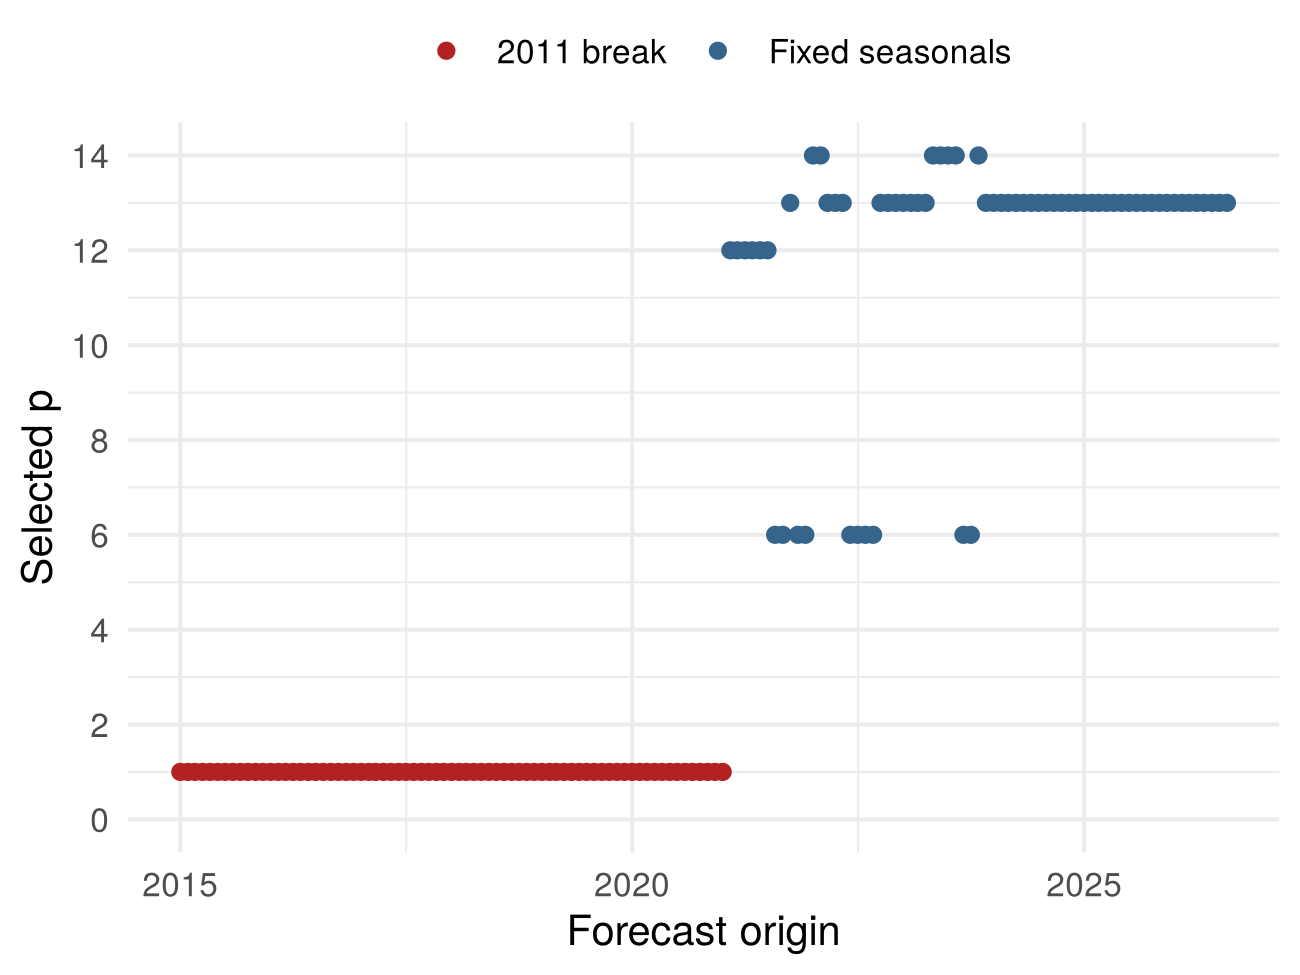
\includegraphics[width=0.49\textwidth]{fig/fig_rule.png}
\caption{Left: out-of-sample RMSPE by horizon (the sample mean is left out because its errors are much larger). Right: lag length and type of seasonal dummies chosen by the selection rule at each forecast origin.}
\label{fig:rmspe}
\end{figure}

The seasonal rule has the lowest RMSPE at every horizon from 1 to 12 months (Table~\ref{tab:rmspe} and Figure~\ref{fig:rmspe}, left). At one month its error is 16\% lower than that of the random walk (0.354 against 0.421). The random walk is a hard benchmark here, and the AR and ARMA models for the annual rate improve on it only a little, because the annual rate is so persistent. The ranking does not depend on the period of high inflation: without 2021-23 the seasonal rule still has the lowest error (0.259). That period does matter for the size of the errors, and so for the width of the forecast intervals in Section~\ref{sec:fc}.

The models chosen by the rule are also informative (Figure~\ref{fig:rmspe}, right). From 2015 to January 2021 the rule selected the 2011 break with one lag. At that time there were only a few years of data after 2011, too few for lags 12 and 13 to learn the new seasonal pattern, and the break captured it directly. From 2021 on, with more years of the new pattern, the rule switched to fixed seasonals with 12 to 14 lags (and $p=6$ in a few months). This is why I kept the break as a candidate even though it does not win today.


I use the RMSPE as a check of the procedure and not to choose the model. Earlier versions of my model with $p\le6$ had slightly lower one-month errors (0.342 with fixed seasonals and 0.346 with the break). With 140 forecast errors, differences of about one hundredth of a point are noise. Choosing the specification with the lowest RMSPE would also use the same data to choose a model and to measure how good it is, which makes the result look better than it really is.

%=====================================================================
\section{The forecast}
\label{sec:fc}

\subsection{Point forecast for October 2026}

With data up to September 2026, the model predicts a monthly change of $\hat m = 0.533\%$ for October. The seasonal part (constant plus the October dummy) contributes 0.068 points. The largest contributions from the lags come from April 2026 through lag 6 (0.269 times 1.02 = 0.275) and from September 2026 through lag 1 (0.253 times 0.60 = 0.151). The same month of 2025 adds 0.060 through lag 12, and the remaining lags together add $-0.021$. The forecast index is $104.31\times e^{0.00533}=104.87$, and with the October 2025 index of 100.74, equation \eqref{eq:rebuild} gives
\[
\hat\pi_{\text{Oct 2026}} = 100\times(104.87/100.74 - 1) = 4.10\%.
\]
Rounded as Eurostat publishes it, \textbf{my forecast is 4.1\%}. The result is consistent with the base effect in \eqref{eq:sum}: prices are expected to rise by 0.53\% this October against 0.22\% in October 2025, which moves the annual rate up by about 0.3 points from 3.8\%.

\textbf{Robustness.} The October forecast hardly depends on the details of the selection rule. Table~\ref{tab:robust} gives it for the selected model and five alternatives: the specification with the best BIC overall (which fails the residual check), the neighbouring lag lengths, the AR(14) that the rule would choose with $R-p$ degrees of freedom, and two models with the 2011 break (the one with the best BIC, $p=6$, and $p=13$). The forecasts go from 4.01\% to 4.15\%. Four of the six round to 4.1\%, and the other two to 4.0\% and 4.2\%. All of these models include lag 6, so the table does not answer the concern about April 2026 that I discuss in Section~\ref{sec:others}. It shows that the choice among reasonable specifications does not change the result.

\begin{table}[htbp]
\centering
\small
\caption{October 2026 forecast under alternative specifications}
\label{tab:robust}
\begin{tabular}{@{}lrrrccr@{}}
\toprule
 & & & & \multicolumn{2}{c}{Passes Box-Pierce with} & \\
\cmidrule(lr){5-6}
Seasonal dummies & $p$ & BIC & $Q(18)$ & $\chi^2(R)$ & $\chi^2(R-p)$ & Forecast (\%)\\
\midrule
Fixed & 6 & $-2.488$ & 29.8 & no & no & 4.10\\
Fixed & 12 & $-2.457$ & 17.8 & yes & no & 4.01\\
\rowcolor{gray!30} Fixed (selected) & 13 & $-2.484$ & 11.7 & yes & no & 4.10\\
Fixed & 14 & $-2.478$ & 7.5 & yes & yes & 4.10\\
2011 break & 6 & $-2.417$ & 19.1 & yes & yes & 4.13\\
2011 break & 13 & $-2.358$ & 10.6 & yes & yes & 4.15\\
\bottomrule
\end{tabular}

\vspace{3pt}
{\footnotesize BIC and $Q$ from Table~\ref{tab:select} (common sample). Forecasts use the full sample.}
\end{table}

\subsection{Forecast intervals}

The intervals are $\hat\pi_{T+h}\pm z\,v_h$, with $z=0.674$ for the 50\% interval and $z=1.645$ for the 90\% interval, which assumes normal forecast errors. Following Handout 4, $v_h$ is the standard deviation of the out-of-sample forecast errors of the selection rule at horizon $h$ (Section~\ref{sec:oos}). For $h=1$, $v_1=0.354$, so the 50\% interval is $4.10\pm0.24$, or 3.9\% to 4.3\%, and the 90\% interval is $4.10\pm0.58$, or 3.5\% to 4.7\%.

As a comparison I also computed $v_h$ from the model, as in the course slides, where $v_h^2=(1+\phi^2+\dots+\phi^{2(h-1)})\sigma^2$ for an AR(1). For my model the error of the annual rate at horizon $h$ is the sum of the monthly errors from $T+1$ to $T+h$, so $v_h^2=\sigma^2\sum_{r=1}^{h}(\psi_0+\dots+\psi_{r-1})^2$, where the $\psi_j$ are the weights that show how a shock today affects the monthly change $j$ months later ($\psi_0=1$, $\psi_1=\phi_1$, and so on). At $h=1$ this is just $\hat\sigma$, adjusted from the log index to the annual rate, $v_1=0.253$, which gives a narrower 90\% interval of 3.7\% to 4.5\%. I use the out-of-sample version because the model-based formula treats the estimated coefficients as known and uses the average residual variance of 1998-2026, while the out-of-sample errors include parameter uncertainty and the large errors of 2021-23.

As a check of the intervals, I counted how many of the out-of-sample errors of Section~\ref{sec:oos} fall inside intervals built in this way. At $h=1$, 62\% of the errors are inside the 50\% interval and 91\% inside the 90\% interval. Over all horizons the shares are 68\% and 90\%. The 90\% intervals have about the right coverage, but the 50\% intervals are too wide. This is what happens when errors have fat tails: the large errors of 2021-23 raise $v_h$, while most errors are small. Without 2021-23 the shares at $h=1$ are 70\% and 96\%, so in a calm month my intervals are probably too wide rather than too narrow. Since $v_h$ comes from the same errors, this is a consistency check and not an independent test.

\subsection{Forecasts for the next twelve months}

Table~\ref{tab:fc} gives the forecasts from October 2026 to September 2027, and Figure~\ref{fig:fan} shows them with the intervals.

\begin{table}[htbp]
\centering
\small
\caption{Forecasts of euro area HICP annual inflation (\%) with 50\% and 90\% intervals}
\label{tab:fc}
\begin{tabular}{@{}lrrrrrr@{}}
\toprule
 & & \multicolumn{2}{c}{50\% interval} & \multicolumn{2}{c}{90\% interval} & \\
\cmidrule(lr){3-4}\cmidrule(lr){5-6}
Month & Forecast & Lower & Upper & Lower & Upper & $v_h$\\
\midrule
\rowcolor{gray!30} October 2026 & \textbf{4.10} & 3.86 & 4.34 & 3.52 & 4.68 & 0.35\\
November 2026 & 4.34 & 3.96 & 4.72 & 3.41 & 5.26 & 0.56\\
December 2026 & 4.35 & 3.86 & 4.84 & 3.15 & 5.55 & 0.73\\
January 2027 & 4.49 & 3.89 & 5.09 & 3.02 & 5.96 & 0.89\\
February 2027 & 4.48 & 3.76 & 5.19 & 2.73 & 6.22 & 1.06\\
March 2027 & 4.28 & 3.45 & 5.11 & 2.26 & 6.31 & 1.23\\
April 2027 & 3.92 & 2.96 & 4.89 & 1.56 & 6.29 & 1.44\\
May 2027 & 3.92 & 2.80 & 5.04 & 1.19 & 6.65 & 1.66\\
June 2027 & 4.10 & 2.84 & 5.36 & 1.04 & 7.16 & 1.86\\
July 2027 & 3.85 & 2.46 & 5.24 & 0.46 & 7.24 & 2.06\\
August 2027 & 3.69 & 2.16 & 5.21 & $-0.04$ & 7.41 & 2.27\\
September 2027 & 3.52 & 1.86 & 5.19 & $-0.53$ & 7.58 & 2.47\\
\bottomrule
\end{tabular}

\vspace{3pt}
{\footnotesize Intervals: forecast $\pm\,z\,v_h$, with $v_h$ the standard deviation of the out-of-sample errors at horizon $h$, $z=0.674$ (50\%) and $z=1.645$ (90\%).}
\end{table}

\begin{figure}[htbp]
\centering
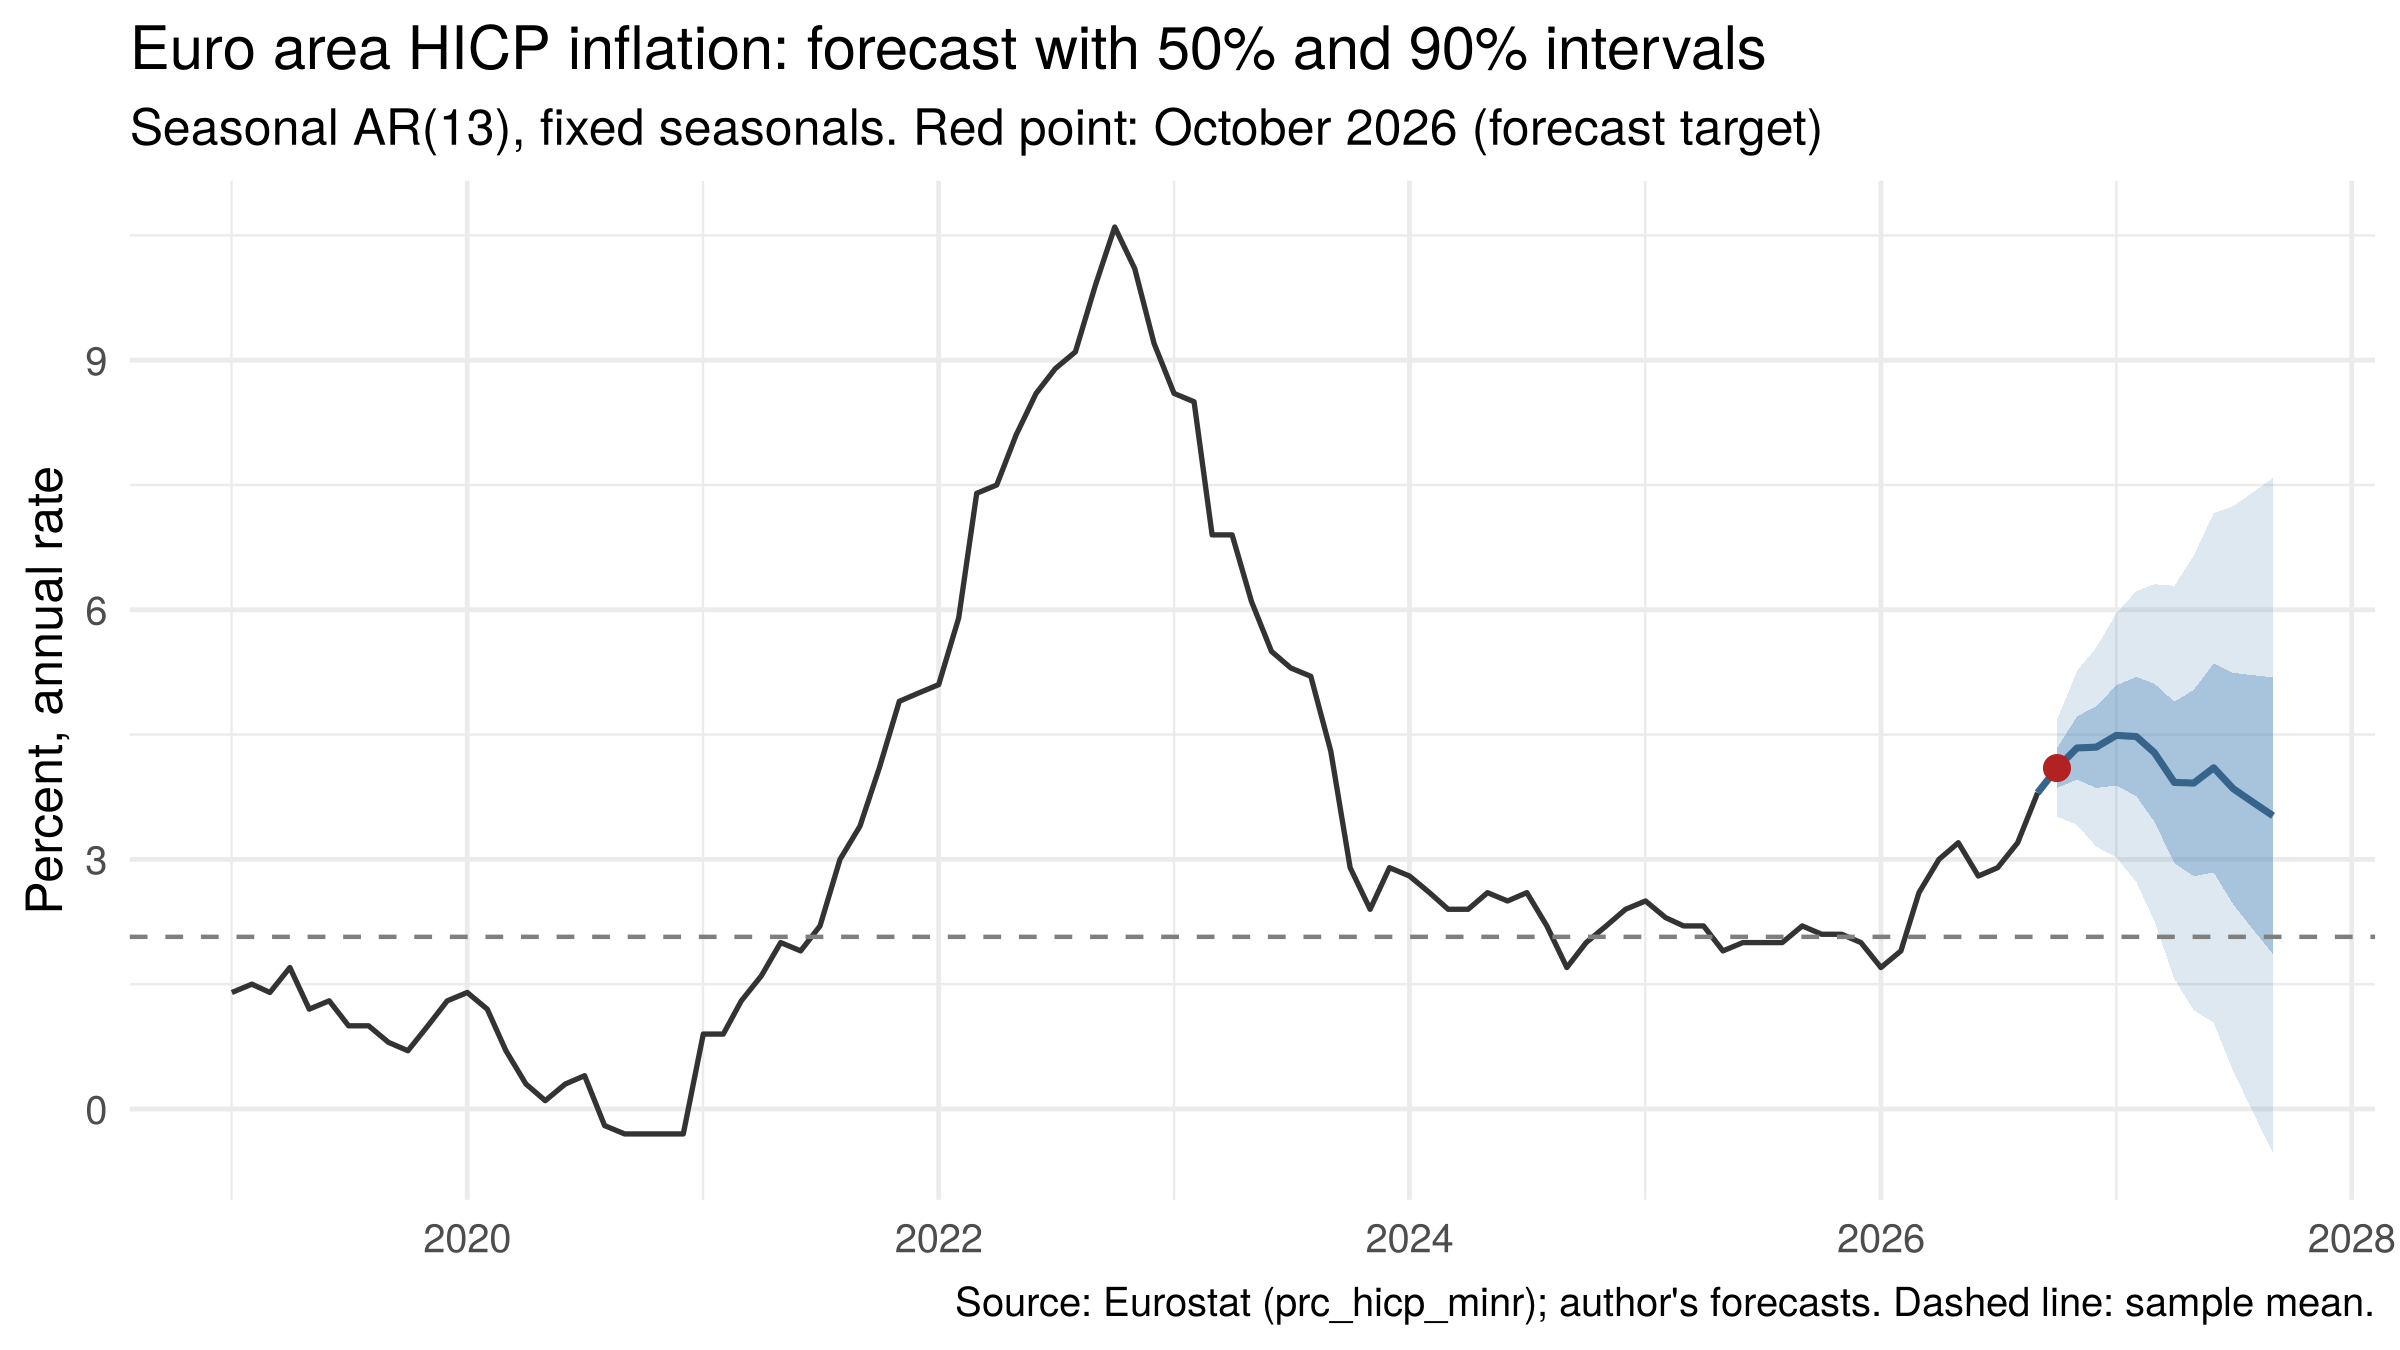
\includegraphics[width=0.8\textwidth]{fig/forecast_fan.png}
\caption{Annual inflation since 2019 and forecasts to September 2027 with 50\% (dark) and 90\% (light) intervals. The red point is the October 2026 target.}
\label{fig:fan}
\end{figure}

The path rises to about 4.5\% in early 2027 and then falls to 3.5\% by September 2027. Both movements are mostly base effects. The last months of 2025 had small price increases, so the annual rate keeps rising as long as the new months rise more. March and April 2026 had very large monthly increases (1.26\% and 1.02\%), and when these months leave the annual rate in 2027, it starts to fall. The intervals widen quickly with the horizon: at 12 months the 90\% interval goes from $-0.5\%$ to 7.6\%. This reflects how volatile inflation was in the evaluation period.

%=====================================================================
\section{Comparison with other forecasts}
\label{sec:others}

Table~\ref{tab:others} compares my forecasts with published forecasts by others.

\begin{table}[htbp]
\centering
\small
\caption{My forecasts and forecasts by others}
\label{tab:others}
\begin{tabularx}{\textwidth}{@{}Xccc@{}}
\toprule
Forecaster (date) & October 2026 & 2026 Q4 average & 2026 annual average\\
\midrule
This paper (November 3, 2026) & 4.1 & 4.3 & 3.2\\
Market consensus, Trading Economics calendar (November 3, 2026) & 4.0 & & \\
Trading Economics model forecast (November 3, 2026) & 3.9 & & \\
BofA Global Research (late October 2026) & 3.7 & & \\
Pantheon Macroeconomics (late October 2026) & 4.0 & & \\
ECB staff projections (September 10, 2026) & & 3.6 & 3.0\\
ECB Survey of Professional Forecasters (October 2 to 7, 2026) & & & 3.0\\
\bottomrule
\end{tabularx}

\vspace{3pt}
{\footnotesize My 2026 average uses actual data for January to September and my forecasts for October to December. Sources are listed in the references.}
\end{table}

For October my forecast of 4.1\% is one decimal above the market consensus of 4.0\% and close to the other forecasts I found, which go from 3.7\% (BofA) to 4.0\% (Pantheon). All of them are inside my 90\% interval, and the consensus is inside my 50\% interval. The difference is larger further out. The ECB staff expected inflation to peak at 3.6\% in the fourth quarter of 2026 and fall to 2.5\% in the second quarter of 2027, while my model has 4.3\% and 4.0\% for these quarters. The ECB projections assume that oil and gas prices fall, in line with futures markets, and they expect energy inflation to turn negative during 2027. My model only uses past inflation, so it cannot see this. It also passes the large increases of March and April 2026, which were partly driven by energy, into later months through lag 6, as the decomposition in Section~\ref{sec:fc} shows. For the one-month forecast this matters less, but it is the main reason to trust the professional forecasts more than mine for 2027.

National flash estimates for October were published on October 30, before this report: annual HICP inflation was 3.8\% in France, 5.6\% in Italy and 4.9\% in Spain, and German CPI inflation was 2.8\% (Euronews, 2026). I did not use them, because the forecast should come only from the model and data described above.

%=====================================================================
\section{Limitations and conclusion}
\label{sec:concl}

The model has several limitations. It is univariate, so it does not use information on energy prices, which drove much of the rise in inflation in 2026 and would probably help at short horizons. It also cannot tell whether a large past increase came from seasonal factors or from energy, which affects the October forecast through lag 6. The intervals depend on the evaluation period, and 2021-23 makes them wide. The evaluation uses the current vintage of the data and not the data available at each origin, although HICP revisions are small. Finally, one choice was made after looking at the data: raising $p_{\max}$ from 6 to 14. I justify it independently of which model wins, because the BIC chose the upper limit and monthly data should allow at least a year of lags.

To summarise, I forecast euro area HICP inflation for October 2026 by modelling the monthly price change with seasonal dummies and an autoregression, and rebuilding the annual rate from the index. The model was chosen by a rule fixed in advance, based on the Box-Pierce test and the BIC, which selected an AR(13) with fixed seasonals. Out of sample, this rule has the lowest RMSPE of the models I compare at every horizon, although at one month the gain over the AR for the annual rate is small (0.354 against 0.374). Alternative specifications give October forecasts between 4.01\% and 4.15\%. My forecast is 4.1\%, with a 50\% interval of 3.9\% to 4.3\% and a 90\% interval of 3.5\% to 4.7\%. A natural extension would be an autoregressive distributed lag model that adds oil and gas prices in euros, evaluated with the same out-of-sample procedure.

%=====================================================================
\section*{References}
\small
\begin{itemize}\setlength{\itemsep}{1pt}
\item[] Box, G. E. P. and Pierce, D. A. (1970). Distribution of residual autocorrelations in autoregressive-integrated moving average time series models. \emph{Journal of the American Statistical Association}, 65(332), 1509-1526.
\item[] Commission Regulation (EC) No 330/2009 of 20 April 2009 laying down detailed rules for the implementation of Council Regulation (EC) No 2494/95 as regards minimum standards for the treatment of seasonal products in the Harmonised Indices of Consumer Prices. \emph{Official Journal of the European Union}, L 103.
\item[] European Central Bank (2026a). \href{https://www.ecb.europa.eu/press/projections/html/ecb.projections202609_ecbstaff~8e340fc69d.en.html}{ECB staff macroeconomic projections for the euro area, September 2026}.
\item[] European Central Bank (2026b). \href{https://www.ecb.europa.eu/stats/ecb_surveys/survey_of_professional_forecasters/html/ecb.spf2026q4.en.html}{The ECB Survey of Professional Forecasters, fourth quarter of 2026}.
\item[] Euronews (2026). \href{https://www.euronews.com/2026/10/30/germany-france-italy-and-spain-where-was-inflation-highest-in-october}{Germany, France, Italy and Spain: where was inflation highest in October?} October 30, 2026.
\item[] Eurostat (2026a). \href{https://ec.europa.eu/eurostat/web/products-euro-indicators/w/2-16102026-ap}{Annual inflation up to 3.8\% in the euro area}. Euro indicators, October 16, 2026.
\item[] Eurostat (2026b). \href{https://ec.europa.eu/eurostat/databrowser/view/prc_hicp_minr/default/table}{HICP: monthly data (index and rates of change), \texttt{prc\_hicp\_minr}}. Retrieved October 2026.
\item[] Lahti, L., Huovari, J., Kainu, M. and Biecek, P. (2017). Retrieval and analysis of Eurostat open data with the eurostat package. \emph{The R Journal}, 9(1), 385-392.
\item[] Trading Economics (2026). \href{https://tradingeconomics.com/euro-area/inflation-cpi}{Euro area inflation rate}. Accessed November 3, 2026.
\item[] West, K. D. (2026). Econ 460 lecture notes and handouts, University of Wisconsin--Madison: lectures 4, 9, 10, 11 and 12, Handouts 2 and 4, and ``2026 forecasts of inflation'' slides.
\end{itemize}
\normalsize

%=====================================================================
\newpage
\appendix
\section*{Appendix: R code}
The script below downloads the data, runs the selection rule, the out-of-sample evaluation and the final forecast, and saves all tables and figures used in this paper. It uses R with the packages \texttt{eurostat}, \texttt{dplyr} and \texttt{ggplot2}.
\lstinputlisting[language=R]{../forecast.R}

\end{document}
